\documentclass[assignment2.tex]{subfiles}
\begin{document}

\section*{3η Άσκηση}
Η συνάρτηση $f(x)=x^4+2x^3-5x^2-7x-5$ στο διάστημα $I=[1.5, 3]$ φαίνεται στο Σχήμα \ref{fig:f3}. Η $f$ είναι γνησίως αύξουσα στο $I$ και ισχύει ότι $f(1.5)f(3)<0$, επομένως η $f(x)=0$ έχει μοναδική λύση στο $I$.
\begin{figure}[hp]
	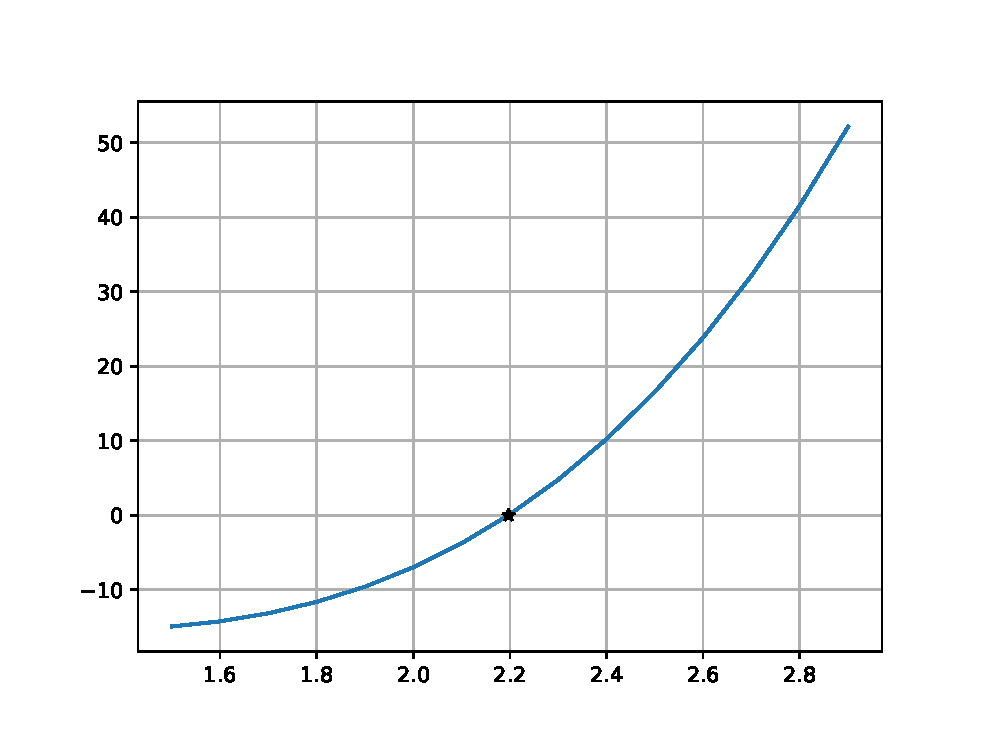
\includegraphics[width=0.7\textwidth]{f3.eps}
	\centering
	\caption{Γράφημα $f(x)=x^4+2x^3-5x^2-7x-5$ στο $I$}
	\label{fig:f3}
\end{figure}

\paragraph{Μέθοδος \textlatin{Newton-Raphson}}
Η μέθοδος \textlatin{Newton-Raphson} συγκλίνει σε ρίζα μιας $f$, δεδομένου ότι η αρχική εκτίμηση $x_0$ είναι αρκετά κοντά στη ρίζα. Η εκτέλεση της μεθόδου έγινε για $x_0=2$ και βρέθηκε η ρίζα $\rho= 2.19714$ μετά από $N=4$ επαναλήψεις.

\paragraph{Μέθοδος εσφαλμένης θέσης}
Η μέθοδος της εσφαλμένης θέσης επίσης συγκλίνει στη ρίζα της $f$ στο $I$, αλλά πιο αργά από την \textlatin{Newton-Raphson}. Συγκεκριμένα, έδωσε $\rho=2.19714$ μετά από $N=8$ επαναλήψεις.

\paragraph{Μέθοδος διχοτόμησης}
Η μέθοδος της διχοτόμησης είναι η πιο αργή από όλες τις μεθόδους και συνέκλινε στην τιμή $\rho=2.19714$ μετά από $N=18$ επαναλήψεις.

Από τη σύγκριση των τριών μεθόδων, η πιο γρήγορη είναι η \textlatin{Newton-Raphson} και ο λόγος είναι ότι η ταχύτητα σύγκλισής της είναι τετραγωνική. Συγκρίνοντας την μέθοδο εσφαλμένης θέσης με αυτή της διχοτόμησης, η πρώτη είναι πιο γρήγορη αλλά όχι πάντα. Στη συγκεκριμένη περίπτωση, είναι αρκετά πιο γρήγορη και μάλιστα για διαφορετική επιλογή $x_0$, η \textlatin{Newton-Raphson} μπορεί να συγκλίνει στον ίδιο αριθμό επαναλήψεων με την μέθοδο εσφαλμένης θέσης. Γενικά, η μέθοδος της διχοτόμησης είναι η πιο αργή, αλλά εγγυάται πάντα τη σύγκλιση σε μια ρίζα μιας συνάρτησης.

Παρακάτω ακολουθεί ο κώδικας που γράφτηκε σε \textlatin{Python} και έγινε χρήση της βιβλιοθήκης \textlatin{Numpy}.
\selectlanguage{english}
\lstinputlisting[style=python, firstline=8]{ex3.py}
\end{document}